\documentclass{article}
\usepackage{amsmath}
\usepackage{amssymb}
\usepackage{enumitem}
\usepackage[style=verbose]{biblatex}
\usepackage[margin=1in]{geometry}
\usepackage{hyperref}
\usepackage{graphicx}

\title{Note 7: Vector and Matrix Calculus}
\author{Math 198: Math for Machine Learning}
\date{}

\begin{document}
\maketitle

\noindent Note on notation: Functions in this section of the course are sometimes described as mapping general topological spaces $\mathcal{X}$ to other topological spaces. $\mathbb{R}^n$ is an example of a topological space; any vector space with an inner product is as well. Therefore, all these definitions and theorems apply to functions on the vector spaces we worked with in the previous section.

\section{Extrema}
As in one-dimensional calculus (by which is meant calculus on functions in one variable), vector calculus is concerned with the rate of change of functions. Recall that in one-dimensional calculus, \textit{critical points} are points at which the rate of change of the function is 0, which are either local/global minima, local/global maxima, or saddle points. Of these, the minima and maxima are labeled \textit{extrema}. Our primary application of vector calculus will be solving optimization problems. For example, we seek the weights $\mathbf{w}$ which minimize the value $\mathbf{||Xw - y}||_2^2$; in other words, the global minimum of the function $f(\mathbf{w}) = ||\mathbf{Xw - y}||_2^2$. To solve this optimization problem, we could attempt to find all the extrema of $f(\mathbf{w})$, and determine which of these is the global minimum. We will later build more sophisticated methods to do this more efficiently; nonetheless, the goal of all of these methods will be to locate extrema. \\\\
For a function $f: \mathcal{X} \rightarrow \mathbb{R}$, we define a vector $\mathbf{x} \in \mathcal{X}$ to be a \textit{local minimum} of $f$ if $f(\mathbf{x}) \leq f(\mathbf{y})$ for all $\mathbf{y}$ in some open set $\mathcal{N} \subseteq \mathcal{X}$ such that $\mathbf{x} \in \mathcal{N}$.\footnote{An open set is loosely a shaded circle on the input space, and an open set containing a particular vector $\mathbf{v}$ is known as a "neighborhood about $\mathbf{v}$".} If $\mathcal{N} = \mathcal{X}$ and the conditions hold, i.e. $\forall \mathbf{y} \in \mathcal{X}$  $f(\mathbf{x}) \leq f(\mathbf{y})$, then $\mathbf{x}$ is a \textit{global minimum} of $f$ in $\mathcal{X}$. A global/local minimum is \textit{strict} if the same conditions hold, except $f(\mathbf{x}) < f(\mathbf{y})$ (the extrema is unique). \\\\
The definitions of local/global maximum proceed similarly, although we generally only consider minima in optimization. This is because maximizing a function $f$ is the same as minimizing $-f$, so all maximization problems can be (and are) rewritten as minimization problems.

\section{Gradients, Jacobians, Hessians}

\subsection{Gradients}
We start by generalizing derivatives to vector calculus. The \textit{gradient} of a function $f: \mathbb{R}^d \rightarrow \mathbb{R}$ is given by $$\nabla f(\mathbf{x}) = \begin{bmatrix} \frac{\partial f}{\partial \mathbf{x}_1} \\ \vdots \\ \frac{\partial f}{\partial \mathbf{x}_d} \end{bmatrix}$$ Therefore, $\nabla f(\mathbf{x}) \in \mathbb{R}^d$; in fact, $\nabla f(\mathbf{x})$ points in the direction of steepest ascent along $f$ from $\mathbf{x}$, and so $-\nabla f(\mathbf{x})$ points in the direction of steepest descent. Additionally, $\nabla f(\mathbf{x}) = \mathbf{0}$ if $\mathbf{x}$ is a critical point. Proofs of these theorems will be covered in Note 9.

\subsection{Jacobians}
We can do the same for derivatives in matrix calculus. Our function $f: \mathbb{R}^n \rightarrow \mathbb{R}^m$ is now a more general linear map (described by a matrix) and its derivative, known as the \textit{Jacobian}, is, too, a matrix: $$\mathbf{J}_f(\mathbf{x}) = \begin{bmatrix} \frac{\partial f}{\partial \mathbf{x}_1} & \hdots & \frac{\partial f}{\partial \mathbf{x}_n} \end{bmatrix} = \begin{bmatrix} \frac{\partial f_1}{\partial \mathbf{x}_1} & \hdots & \frac{\partial f_1}{\partial \mathbf{x}_n} \\ \vdots & \ddots & \vdots \\ \frac{\partial f_m}{\partial \mathbf{x}_1} & \hdots & \frac{\partial f_m}{\partial \mathbf{x}_n} \end{bmatrix}$$ In the case that $m = 1$, then $\mathbf{J}_f = \nabla f^{\top}$.

\subsection{Hessians}
The \textit{Hessian} generalizes second-order derivatives to vector calculus.\footnote{The second derivative in matrix calculus must be represented as a \textit{tensor}, the higher-dimensional generalization of a matrix, and is not covered in this class.} It is the matrix of second-order partial derivatives: $$\nabla^2f(\mathbf{x}) = \begin{bmatrix} \frac{\partial^2f}{\partial \mathbf{x}_1\partial\mathbf{x}_1} & \hdots & \frac{\partial^2f}{\partial\mathbf{x}_1\partial\mathbf{x}_d} \\ \vdots & \ddots & \vdots \\ \frac{\partial^2f}{\partial \mathbf{x}_d\partial\mathbf{x}_1} & \hdots & \frac{\partial^2f}{\partial\mathbf{x}_d\partial\mathbf{x}_d} \end{bmatrix}$$ If the partial derivatives are continuous, the order of differentiation can be interchanged, as in one-dimensional calculus. Therefore, in this case, the Hessian is symmetric.

\subsection{Differentiation Rules}
We introduce the following useful rules for differentiation around vectors and matrices: $$\nabla_{\mathbf{x}}(\mathbf{a}^{\top}\mathbf{x}) = \mathbf{a}$$ and if $\mathbf{A}$ is square, $$\nabla_{\mathbf{x}}(\mathbf{x}^{\top}\mathbf{Ax}) = \mathbf{(A + A^{\top})x}$$ These identities are not valid if the values of $\mathbf{a}$ or $\mathbf{A}$ depend on $\mathbf{x}$. However, the chain rule still holds. If we have $f: \mathbb{R}^m \rightarrow \mathbb{R}^k$ and $g: \mathbb{R}^n \rightarrow \mathbb{R}^m$, then $f \circ g: \mathbb{R}^n \rightarrow \mathbb{R}^k$ and $$\mathbf{J}_{f \circ g}(\mathbf{X}) = \mathbf{J}_f(g(\mathbf{x}))\mathbf{J}_g(\mathbf{x})$$ If $k = 1$ then $$\nabla (f \circ g)(\mathbf{x}) = \mathbf{J}_g(\mathbf{x})^{\top}\nabla f(g(\mathbf{x}))$$ The proofs follow easily from the chain rule on partial derivatives.

\clearpage

\section*{Applications: Gradient Descent}
All of our models so far have been linear regression models, i.e. they find weights $\mathbf{w}$ such that the output $y$ can be expressed as a linear combination of the input $\mathbf{x}$. This has been the case even when working with non-linear features, as we augmented the features prior to finding the weights. As we will prove in the next note, linear models have particular nice properties which allow us to find closed-form solutions (i.e. $\mathbf{w} = (\mathbf{X^{\top}X})^{-1}\mathbf{X^{\top}y}$). However, we are not always able to find closed-form solutions for non-linear models. It would be nice to have a method which could approximate solutions for functions for which no closed-form solutions exist. Furthermore, in some applications, we don't even know what type of function we are trying to approximate -- we instead use a \textit{universal function approximator} capable of approximating arbitrary functions. \textit{Neural networks}, mathematical objects loosely based on the brain's neural structures, are one such universal function approximator which use large quantities of weights as well as non-linear functions to learn arbitrary function. Because no closed-form solution exists to find the correct weights, we instead turn to the \textit{gradient descent} algorithm, which attempts to find local minima in the objective function of the model. Recall from section 2.1 that the gradient of a function points in the direction of steepest ascent. Therefore, like a ball rolling down a hill, the gradient descent algorithm repeatedly takes steps along the negative of the gradient in an attempt to find nearby local minima. However, note that at critical points, the gradient is 0. Therefore, this algorithm cannot find the global minima of functions, as it will stop taking further steps once it reaches a local minima (or saddle point, although this rarely happens in practice). Nonetheless, its strength is in the fact that it works for \textbf{any} objective function, even when no closed-form solution exists.\footnote{We will discuss other such methods in Note 9; however, gradient descent is the most widely used, so we're introducing it a bit ahead of schedule.}\\\\
Recall from Note 1 that the objective function of ordinary least squares is $$L(\mathbf{w}) = \sum\limits_{i=1}^n (y_i - \mathbf{w^{\top}x}_i)^2 = ||\mathbf{y - Xw}||_2^2$$ and we wish to find $\mathbf{w^*}$ which minimizes $L(\mathbf{w})$. In general, our objective function is $$L(\mathbf{w}) = \sum\limits_{i=1}^n (y_i - f(\mathbf{x}_i;\mathbf{w}))^2$$ where $f$ is some arbitrary function \textit{parameterized} by $\mathbf{w}$.\footnote{For example, a cubic polynomial $ax^3 + bx^2 + cx + d$ is parameterized by the vector $[a, b, c, d]$. A function $f(\mathbf{x})$ parameterized by a vector $\mathbf{w}$ is expressed notationally as $f(\mathbf{x};\mathbf{w})$.} In the case of linear regression, $f(\mathbf{x}_i; \mathbf{w}) = \mathbf{w^{\top}x}_i$. Note that $\mathbf{X}$ and $\mathbf{y}$ are treated as constants, and so $L$ is only in terms of $\mathbf{w}$. $L$ is often referred to as the \textit{loss/cost function}, as we seek to minimize loss/cost. The gradient descent algorithm works by taking the gradient of the loss function with respect to the current weights, $\nabla L(\mathbf{w})$, and moving the weights in the direction of steepest descent, $-\nabla L$. \\\\
So, the steps of gradient descent are as follows:
\begin{enumerate}[label=\arabic*.]
\item Initialize $\mathbf{w}^{(0)}$ randomly
\item While $L(\mathbf{w}^{(t)})$ has not converged:
		 \begin{enumerate}[label=(\alph*)]
		 \item Update weights: $\mathbf{w}^{(t+1)} = \mathbf{w}^{(t)} - \alpha_t\nabla L_{\mathbf{w}}(\mathbf{w}^{(t)})$
		 \end{enumerate}
\end{enumerate}
On each step, we update the weights by moving down the gradient as scaled by some factor $\alpha_t$, often referred to as the \textit{learning rate}. Like $\lambda$ in ridge regression, the learning rate is a hyperparameter which is not learned by the algorithm and must be set by the user. The learning rate can be constant or can change with the number of iterations -- high learning rates may take steps which are too large and never converge, whereas low learning rates may fail to reach minima because the steps they take are too small. The best method for a particular problem must be determined by \textit{validation}, in which different methods are compared by their loss on unseen data not used in gradient descent. \\\\
The gradient descent algorithm stops when the value of $L(\mathbf{w}^{(t)})$ converges. If $L(\mathbf{w}^{(t)})$ has converged, then $\nabla L(\mathbf{w^{(t)}}) = 0$; therefore, gradient descent is an algorithm for finding critical points, as expected. Gradient descent will certainly not converge to a maxima (unless it starts at one), as it lowers the value of $L(\mathbf{w}^{(t)})$ at each step; additionally, it will almost certainly avoid saddle points unless the gradient around them is very small in all directions, as usually the steps will overshoot saddle points. (The magnitude of the gradient is not necessarily the distance to a critical point; we are only given the direction of steepest descent.) So we expect that gradient descent will mostly return minima -- even if it initially overshoots a local minimum, the direction of steepest descent will reverse, and the algorithm will head back in the right direction. However, once gradient descent finds a local minimum, it will likely get stuck; it will not explore further to find potentially better local minima. Therefore, the quality of the solution returned depends on the initial starting point of the algorithm:

\begin{center}
    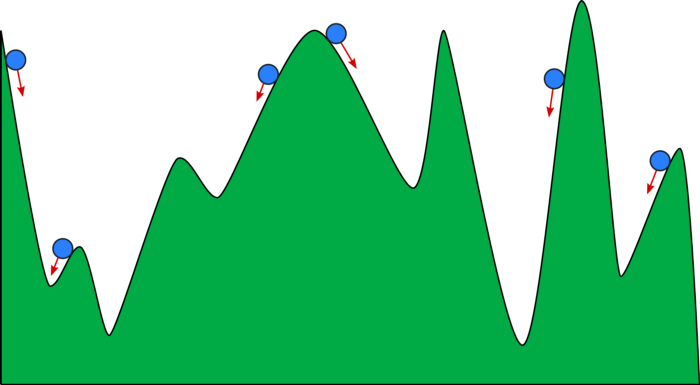
\includegraphics[width=.6\textwidth]{figures/fig1.png}\\
    Source: \href{https://towardsdatascience.com/machine-learning-101-an-intuitive-introduction-to-gradient-descent-366b77b52645}{Towards Data Science}
\end{center}

\noindent Only one of the initializations shown finds the true global minimum, although some are better than others. Nonetheless, gradient descent is very successful at training neural networks, and there are extensions to the algorithm which have better practical performance. However, for a special class of functions, we can show that all local minima are equal to the global minimum. These functions are known as \textit{convex functions}, and we will discuss them in the next note.

\end{document}